% \title{Apunte de Matemáticas Discretas CC3101:\\ 
%   Árboles generadores Clase 23}
% % \title{Ejercicios Lógica e Inducción}
% \author{Andrés Abeliuk}
% \date{}
% \maketitle

\section{Árboles Generadores}

\subsection{Motivación: Conectividad Mínima}

Supongamos que tenemos una red vial entre varias ciudades, en la que todas las rutas son caminos de tierra. Queremos pavimentar la menor cantidad posible de caminos, de modo que sea posible viajar entre cualquier par de ciudades usando sólo caminos pavimentados.

\begin{center}
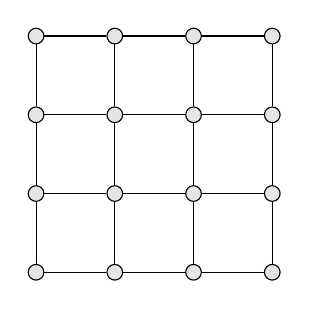
\begin{tikzpicture}[scale=1, every node/.style={circle, draw, fill=gray!20, inner sep=2pt}]
  \foreach \i in {0,...,3} {
    \foreach \j in {0,...,3} {
      \node (v\i\j) at (\i,\j) {};
    }
  }
  \foreach \i in {0,...,3} {
    \foreach \j in {0,...,2} {
      \draw (v\i\j) -- (v\i\the\numexpr\j+1\relax);
    }
  }
  \foreach \i in {0,...,2} {
    \foreach \j in {0,...,3} {
      \draw (v\i\j) -- (v\the\numexpr\i+1\relax\j);
    }
  }
\end{tikzpicture}
\end{center}


\textbf{Pregunta:} ¿Cuál es la mínima cantidad de caminos que deben pavimentarse?


\medskip

La respuesta está dada por encontrar un subgrafo que conecte todas las ciudades (vértices) y no tenga ciclos. Este subgrafo es un \textbf{árbol generador} del grafo original.

\begin{center}
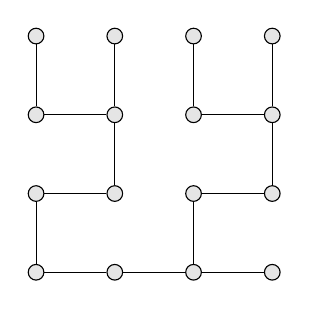
\begin{tikzpicture}[scale=1, every node/.style={circle, draw, fill=gray!20, inner sep=2pt}]
  \foreach \i in {0,...,3} {
    \foreach \j in {0,...,3} {
      \node (v\i\j) at (\i,\j) {};
    }
  }
  \draw (v00) -- (v01);
  \draw (v01) -- (v11);
  \draw (v11) -- (v12);
  \draw (v12) -- (v13);
  \draw (v12) -- (v02);
  \draw (v02) -- (v03);
  \draw (v00) -- (v10); 
  \draw (v10) -- (v20);
  \draw (v20) -- (v30); 
  \draw (v20) -- (v21);
  \draw (v21) -- (v31);
  \draw (v31) -- (v32);
  \draw (v32) -- (v33);
  \draw (v32) -- (v22);
  \draw (v22) -- (v23);
\end{tikzpicture}
\end{center}

\begin{definitionblock}{Árbol Generador}
Un \textbf{árbol generador} de un grafo $G = (V, E)$ es un subgrafo $T = (V, E')$ tal que:
\begin{itemize}
  \item $T$ contiene todos los vértices de $G$, es decir, $V(T) = V(G)$.
  \item $T$ es un árbol: está conectado y no contiene ciclos.
\end{itemize}
\end{definitionblock}


Este tipo de subgrafo no es único: un mismo grafo puede admitir múltiples árboles generadores diferentes, dependiendo de qué aristas se elijan para mantener la conectividad y evitar los ciclos.


\begin{exampleblock}{Ejemplo: Dos árboles generadores distintos del mismo grafo. }

\begin{center}
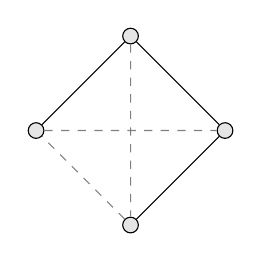
\begin{tikzpicture}[scale=1.2, every node/.style={circle, draw, fill=gray!20, inner sep=2pt}]
  \node (a) at (0,1) {};
  \node (b) at (1,2) {};
  \node (c) at (2,1) {};
  \node (d) at (1,0) {};

  \draw (a) -- (b);
  \draw (b) -- (c);
  \draw (c) -- (d);
  \draw[dashed, gray] (b) -- (d);
  \draw[dashed, gray] (d) -- (a);
  \draw[dashed, gray] (a) -- (c);
\end{tikzpicture}
\hspace{1cm}
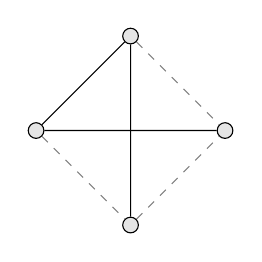
\begin{tikzpicture}[scale=1.2, every node/.style={circle, draw, fill=gray!20, inner sep=2pt}]
  \node (a) at (0,1) {};
  \node (b) at (1,2) {};
  \node (c) at (2,1) {};
  \node (d) at (1,0) {};

  \draw (a) -- (b);
  \draw (b) -- (d);
  \draw[dashed, gray] (d) -- (c);
  \draw[dashed, gray] (a) -- (d);
  \draw (c) -- (a);
  \draw[dashed, gray] (b) -- (c);
\end{tikzpicture}
\end{center}
\end{exampleblock}

\medskip

\begin{center}
  % \includegraphics[width=0.5\textwidth]{SpanningTreeExample.png}
\end{center}

\subsubsection{Aplicación: Recorrido Eficiente}

Una aplicación clave de los árboles generadores es la de recorrer todos los vértices de un grafo de forma eficiente. Por ejemplo, un \textit{rastreador web} (web crawler), que recolecta datos para un motor de búsqueda, necesita visitar todos los documentos conectados por hipervínculos. Para lograrlo de manera eficiente, puede construirse un árbol generador del grafo de enlaces: este árbol permite visitar cada nodo exactamente una vez, garantizando así un recorrido completo en \textbf{tiempo lineal} respecto al número de vértices.



\subsection{Caracterización de Grafos que Admiten Árbol Generador}

Una vez comprendida la noción de árbol generador y su importancia para garantizar conectividad mínima sin redundancia, surge una pregunta natural: ¿qué condiciones debe cumplir un grafo para que sea posible extraerle un árbol generador? 


\begin{thmblock}{Teorema}
Un grafo $G$ admite un árbol generador si y sólo si es conexo.
\end{thmblock}

\begin{proof}
\textbf{($\Rightarrow$)} Si $G$ tiene un árbol generador, entonces $G$ debe ser conexo, porque un árbol conecta todos los vértices por definición.

\medskip

\textbf{($\Leftarrow$)} Sea $G$ un grafo conexo. Si $G$ ya es un árbol, entonces el resultado es inmediato. Si $G$ no es un árbol, entonces contiene al menos un ciclo simple. Podemos remover una arista de ese ciclo sin desconectar el grafo (porque sigue existiendo un camino entre los extremos de esa arista usando el resto del ciclo).

\medskip

Repetimos este proceso mientras haya ciclos: eliminamos una arista de algún ciclo simple. Este proceso debe terminar porque $G$ tiene un número finito de aristas, y cada vez eliminamos una. El resultado final es un subgrafo conexo sin ciclos, es decir, un árbol generador de $G$.
\end{proof}



\subsection{Construcción de Árboles Generadores}

La prueba anterior nos entrega un procedimiento para construir árboles generadores. Sin embargo, este método no es muy eficiente, ya que requiere identificar ciclos simples dentro del grafo. Afortunadamente, existen algoritmos más eficientes y ampliamente utilizados en la práctica para este propósito. Los más conocidos son:

\begin{itemize}
  \item \textbf{DFS (Depth First Search):} búsqueda en profundidad.
  \item \textbf{BFS (Breadth First Search):} búsqueda a lo ancho.
\end{itemize}

\subsubsection{Búsqueda en Profundidad (DFS)}

Dado un grafo no dirigido simple $G$, el algoritmo DFS parte desde un vértice inicial y avanza lo más lejos posible por cada rama antes de retroceder (\emph{backtracking}). De esta forma, se construye un camino largo sin repetir vértices hasta que ya no se pueda continuar, y luego se regresa al nodo anterior para explorar otras ramas.

\begin{center}
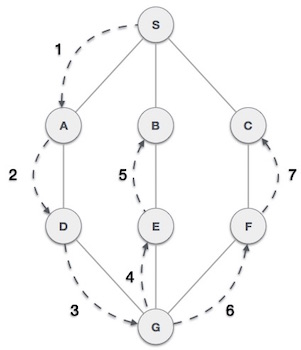
\includegraphics[width=0.25\textwidth]{Figures/DFS1.jpg}
\end{center}



\begin{exampleblock}{Algoritmo DFS}
\textbf{DFS}($G$ grafo conectado con vértices $v_1, v_2, \dots, v_n$):
\begin{itemize}
  \item[] $T$ := árbol que contiene solo el vértice $v_1$
  \item[] visita($v_1$)
\end{itemize}

\textbf{visita}($v$ vértice de $G$):
\begin{itemize}
  \item[] Para cada vértice $w$ adyacente a $v$ y no en $T$ hacer
  \begin{itemize}
    \item[] agregar $w$ y la arista $(v, w)$ a $T$
    \item[] visita($w$)
  \end{itemize}
\end{itemize}
\end{exampleblock}


\subsubsection*{Complejidad del DFS}

\begin{itemize}
  \item Cada vértice $v$ es visitado exactamente una vez: se llama al procedimiento \texttt{visita($v$)} cuando $v$ se encuentra por primera vez.
  \item Cada arista se examina como máximo dos veces: una desde cada uno de sus extremos.
  \item Por lo tanto, DFS tiene complejidad temporal $O(e)$ en representación por listas de adyacencia, o $O(n^2)$ en representación por matrices, donde $n$ es el número de vértices y $e$ el número de aristas.
\end{itemize}

\subsubsection{Búsqueda a lo Ancho (BFS)}

El algoritmo de búsqueda a lo ancho (BFS) también permite construir árboles generadores en grafos conexos. A diferencia del DFS, que explora lo más profundo posible antes de retroceder, el BFS explora todos los vecinos inmediatos de un nodo antes de continuar con los vecinos de esos vecinos, nivel por nivel.

\begin{center}
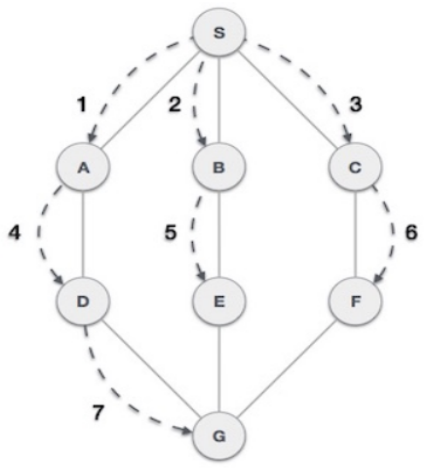
\includegraphics[width=0.25\textwidth]{Figures/BFS1.png}
\end{center}


\begin{exampleblock}{Algoritmo BFS}
\textbf{BFS}($G$ grafo conectado con vértices $v_1, v_2, \dots, v_n$):
\begin{itemize}
  \item[] $T$ := árbol que contiene solo el vértice $v_1$
  \item[] $Q$ := cola que contiene inicialmente solo $v_1$
  \item[] Mientras $Q$ no esté vacía hacer:
  \begin{itemize}
    \item[] $v$ := extraer primer elemento de $Q$
    \item[] Para cada vértice $w$ adyacente a $v$ y no en $T$ hacer
    \begin{itemize}
      \item[] agregar $w$ y la arista $(v, w)$ a $T$
      \item[] insertar $w$ al final de $Q$
    \end{itemize}
  \end{itemize}
\end{itemize}
\end{exampleblock}


\subsubsection*{Complejidad del BFS}

De manera análoga al análisis de DFS:

\begin{itemize}
  \item Cada vértice se visita exactamente una vez.
  \item Cada arista se examina como máximo dos veces: una vez desde cada uno de sus extremos.
  \item Por lo tanto, el algoritmo BFS también tiene una complejidad de $O(e)$ en representación con listas de adyacencia, o $O(n^2)$ con matrices de adyacencia, siendo $n$ el número de vértices y $e$ el número de aristas.
\end{itemize}


\subsection{Ejercicios Propuestos}

\begin{itemize}
  \item \textbf{Ejercicio:} Describa los árboles generadores producidos por los algoritmos DFS y BFS en una rueda $W_n$, comenzando por el vértice central.\\
  Una rueda $W_n$ es un grafo con $n$ vértices que se forma conectando un único vértice a todos los vértices de un ciclo-$(n-1)$.

  \item \textbf{Ejercicio:} Describa los árboles generadores producidos por los algoritmos DFS y BFS en un grafo completo $K_n$.

  \item \textbf{Ejercicio:} Sean $T$ y $T'$ dos árboles generadores del mismo grafo simple $G$. Asuma que existe un arco $e$ en $T$ que no pertenece a $T'$. Demuestre que existe un arco $e'$ en $T'$ tal que $e'$ no está en $T$, y tal que $T$ continúa siendo un spanning tree si le sacamos a $e$ y le agregamos a $e'$, y $T'$ continúa siendo un spanning tree si le sacamos a $e'$ y le agregamos a $e$.
\end{itemize}


\section{Árboles Generadores de Costo Mínimo}

\subsection{Definición y Motivación}

Si un grafo $G$ tiene costos asociados a cada arista, un problema natural es encontrar un árbol generador de \textbf{peso mínimo}. Esto significa hallar un subconjunto acíclico de aristas que conecte todos los vértices y cuya suma de pesos sea mínima.

\begin{definitionblock}{Árbol Generador de Peso Mínimo}
Dado un grafo simple $G$, un \textbf{árbol generador de peso mínimo} es un árbol generador de $G$ tal que la suma de los pesos de sus aristas es mínima.
\end{definitionblock}

\begin{center}
\tikzstyle{vertex}=[circle,fill=black!25,minimum size=20pt,inner sep=0pt]
\tikzstyle{selected vertex} = [vertex, fill=red!24]
\tikzstyle{edge} = [draw,thick,-]
\tikzstyle{weight} = [font=\small]
\tikzstyle{selected edge} = [draw,line width=5pt,-,red!50]
\tikzstyle{ignored edge} = [draw,line width=5pt,-,black!20]

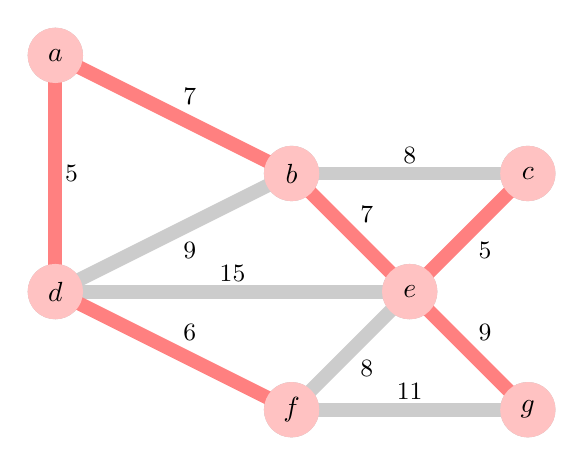
\begin{tikzpicture}[scale=1.5, auto,swap]
    \foreach \pos/\name in {{(0,2)/a}, {(2,1)/b}, {(4,1)/c},
                            {(0,0)/d}, {(3,0)/e}, {(2,-1)/f}, {(4,-1)/g}}
        \node[vertex] (\name) at \pos {$\name$};

    % Edges (ignored first)
    \foreach \source / \dest in {d/b,d/e,e/f,b/c,f/g}
        \path[ignored edge] (\source.center) -- (\dest.center);

    % Edges (selected)
    \foreach \source / \dest in {d/a,d/f,a/b,b/e,e/c,e/g}
        \path[selected edge] (\source.center) -- (\dest.center);

    % Weights on top of everything
    \foreach \source/ \dest /\weight in {b/a/7, c/b/8,d/a/5,d/b/9,
                                         e/b/7, e/c/5,e/d/15,
                                         f/d/6,f/e/8,
                                         g/e/9,g/f/11}
        \path (\source) -- node[weight] {\weight} (\dest);

    % Selected vertices
    \foreach \vertex / \fr in {d/1,a/2,f/3,b/4,e/5,c/6,g/7}
        \node[selected vertex] at (\vertex) {$\vertex$};
\end{tikzpicture}
\end{center}


Hay dos algoritmos clásicos para encontrar árboles generadores mínimos: \textbf{Prim} y \textbf{Kruskal}.

\subsection{Algoritmo de Prim}

\begin{exampleblock}{Algoritmo de Prim}
Dado un grafo simple $G=(V,E)$, $n=|V|$, calcular el árbol de costo mínimo como sigue:
\begin{enumerate}
  \item Escoger el arco de \emph{menor peso} e incluirlo en el árbol.
  \item Repetidamente escoger el arco de menor peso incidente a un vértice existente del árbol, sin formar ciclos.
  \item Repetir hasta obtener $n-1$ aristas.
\end{enumerate}
\end{exampleblock}


\begin{center}
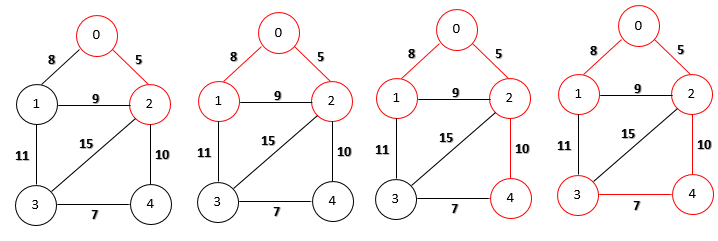
\includegraphics[scale=0.7]{Figures/Prim.png}
\end{center}



\subsection{Algoritmo de Kruskal}

\begin{exampleblock}{Algoritmo de Kruskal}
Dado un grafo simple $G=(V,E)$, $n=|V|$, calcular el árbol de costo mínimo como sigue:
\begin{enumerate}
  \item Ordenar las aristas por peso creciente.
  \item Añadir aristas una a una al árbol si no forman ciclos.
  \item Detenerse al obtener $n-1$ aristas.
\end{enumerate}
\end{exampleblock}

\begin{center}
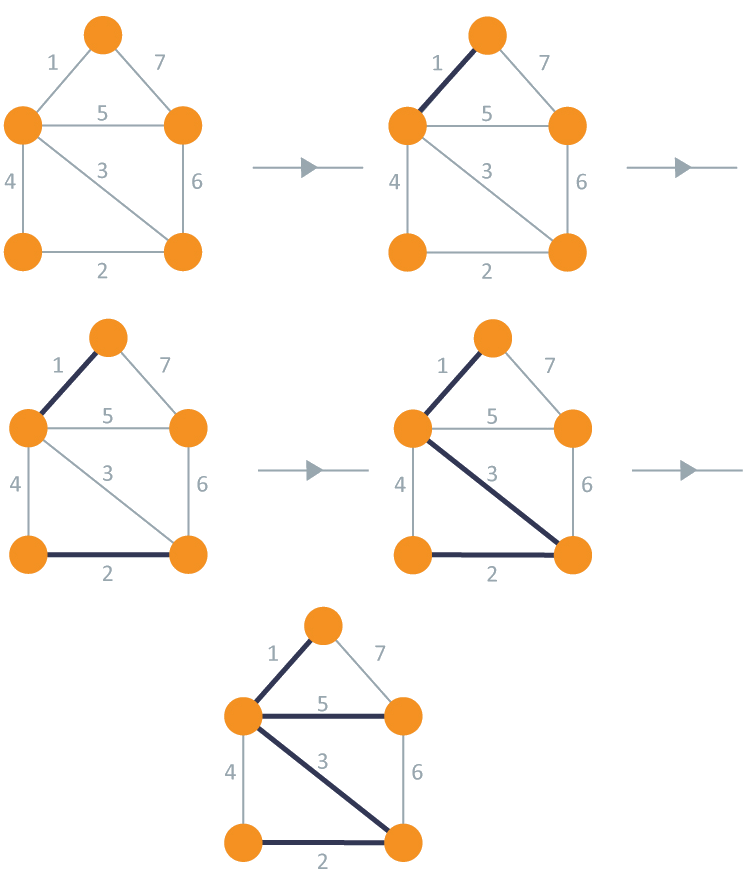
\includegraphics[scale=0.3]{Figures/Kruskal.png}
\end{center}


\subsection{Correctitud de los algoritmos}

Tanto Prim como Kruskal garantizan encontrar un árbol generador de peso mínimo. Sus demostraciones se basan en el principio del intercambio: si una arista no está en el árbol mínimo pero puede reemplazar otra sin aumentar el peso total, entonces el nuevo árbol sigue siendo mínimo.



\begin{thmblock}{Teorema (correctitud algoritmo Prim)}
 Dado un grafo simple $G=(V,E)$ de $n=|V|$ vértices y $e=|E|$ arcos, 
  el algoritmo de Prim encuentra un árbol generador de peso mínimo.
\end{thmblock}
\begin{proof}
Mostraremos la correctitud del algoritmo de Prim usando inducción matemática. Sea $T$ el conjunto de aristas seleccionadas por el algoritmo de Prim en cada iteración, y sea $M$ un árbol generador mínimo (MST).

\textbf{Hipótesis inductiva:} Después de cada iteración, el árbol parcial $T$ es un subgrafo de algún MST $M$.

\textbf{Caso base:} Al inicio, $T = \emptyset$, por lo tanto $T$ es un subgrafo de cualquier MST.

\textbf{Paso inductivo:} Supongamos que antes de una iteración, el árbol parcial $T$ es subgrafo de un MST $M$. Sea $e = (u,v)$ la arista que el algoritmo de Prim selecciona para agregar a $T$ en esta iteración. Como Prim solo añade aristas que conectan un vértice en $T$ con uno fuera, entonces $e$ conecta $T$ con el resto del grafo.

\begin{itemize}
  \item Si $e \in M$, entonces $T \cup \{e\}$ sigue siendo subgrafo de $M$, y la hipótesis se mantiene.
  \item Si $e \notin M$, entonces al agregar $e$ a $M$ se forma un ciclo, ya que $M$ es un árbol.
  \item En ese ciclo, debe existir otra arista $f$ que también conecta un vértice en $T$ con otro fuera de $T$.
  \item Como Prim eligió $e$ en vez de $f$, debe cumplirse que $w(e) \leq w(f)$.
  \item Al eliminar $f$ del ciclo y agregar $e$, obtenemos un nuevo árbol generador $M'$ cuyo peso total es menor o igual al de $M$, y que contiene a $T \cup \{e\}$.
\end{itemize}

Por lo tanto, por inducción, el árbol construido por Prim es un subgrafo de algún MST en cada paso, y al finalizar tiene $n-1$ aristas y conecta todos los nodos. Así, el árbol resultante es un MST.

\end{proof}



% \begin{proof}
% Sea $Y = e_1, \ldots, e_{n-1}$ el árbol generado por el algoritmo de Prim y sea $Y_1$ un árbol generador mínimo (MST).

% Si $Y \neq Y_1$, consideremos $e_k$ como la primera arista añadida durante la construcción de $Y$ que no pertenece a $Y_1$. Entonces, $Y_1$ contiene $e_1, \ldots, e_{k-1}$ pero no $e_k$.

% Sea $V$ el conjunto de vértices conectados por las aristas añadidas antes de $e_k$. Un extremo de $e_k$ está en $V$ y el otro fuera. Como $Y_1$ es un MST, existe un camino en $Y_1$ entre los extremos de $e_k$, y por lo tanto existe una arista $f$ en $Y_1$ que conecta $V$ con su complemento.

% En la iteración donde se eligió $e_k$, también se podría haber elegido $f$, lo cual implica:
% \[
%   w(f) \geq w(e_k)
% \]

% Sea $Y_2$ el grafo obtenido al reemplazar $f$ por $e_k$ en $Y_1$. Este nuevo grafo es también un árbol generador con peso total menor o igual al de $Y_1$, y contiene $e_k$. Repitiendo este procedimiento, obtenemos un MST que es idéntico al árbol $Y$.
% \end{proof}



\begin{thmblock}{Teorema (correctitud algoritmo Kruskal)}
Dado un grafo simple $G=(V,E)$ de $n=|V|$ vértices y $e=|E|$ arcos, 
  el algoritmo de Kruskal encuentra un árbol generador de peso mínimo.
\end{thmblock}

\paragraph{Propuesto: Demostrar correctitud del Algoritmo de Kruskal.}
La demostración de correctitud del algoritmo de Kruskal se basa en un argumento inductivo, similar al de Prim.

\subsection{Complejidad Algoritmos de Prim y Kruskal}

Dado un grafo simple $G = (V, E)$, el costo computacional de cada algoritmo es:

\begin{itemize}
  \item \textbf{Prim:} \stitle{$O(|E| \log |V|)$} \,\, (usando una cola de prioridad).
  \item \textbf{Kruskal:} \stitle{$O(|E| \log |E|)$} \,\, (ordenamiento de aristas y estructura de conjuntos disjuntos).
\end{itemize}


\textbf{¿Cuándo conviene usar Kruskal?} Cuando el grafo es esparso, es decir, cuando el número de aristas es relativamente pequeño comparado con el número de vértices. En estos casos, Kruskal tiende a ser más rápido porque requiere considerar menos aristas y su estructura de datos es más simple que la de Prim con cola de prioridad.

